
\section{Introduction}
Exchange is basically a mail server that supports a bunch of Microsoft protocols. It’s usually located on subdomains named autodiscover, mx, owa or mail, and it can also be detected by existing /owa/, /ews/, /ecp/, /oab/, /autodiscover/, /Microsoft-Server-ActiveSync/, /rpc/, /powershell/ endpoints on the web server.

\begin{figure}[!ht]
  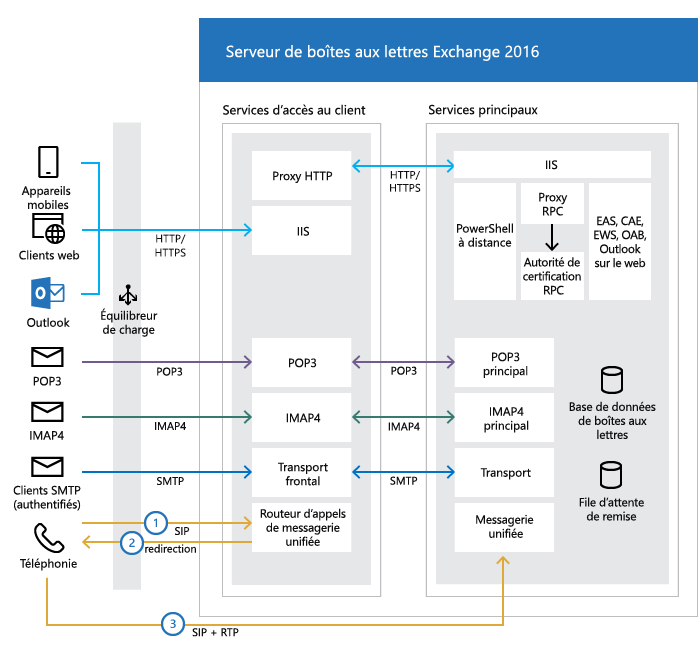
\includegraphics[width=\linewidth]{network/exchange/images/archi.png}
    \caption{Exchange Archi}
  \label{fig:exchange-archi}
\end{figure}


Exchange has a few remote access protocols that we can abuse:
\begin{itemize}
    \item 
        {\bf Exchange Web Services (EWS)} is essentially SOAP over HTTP that lets applications access items in a Microsoft Exchange email mailbox, such as calendars, contacts and messages 
    \item
        {\bf Outlook Anywhere} is sort of EWS predecessor, essentially RPC over HTTP or sub-protocols underneath RPC over HTTP, for example MAPI over RPC over HTTP.
    \item
        {\bf Messaging Application Programming Interface (MAPI)}As of Exchange 2013, Microsoft gave up on RPC and uses straight MAPI over HTTP. Subsequently, Office365, Outlook.com and any Exchange 2013+ servers typically support direct MAPI over HTTP.
    \item
        {\bf Exchange ActiveSync (EAS)}, which is an older protocol using HTTP and XML. EAS is typically used for older mobile devices, since it is a high latency/low bandwidth network protocol. It can be abused to access assets that are out of our reach.
    \item
        {\bf Name Service Provider Interface (NSPI) Protocol} which is 
used by Messaging API (MAPI) clients to access the directory service. This interface is a component of the Exchange Server architecture and is used for addressing and name resolution within the Exchange environment. The NSPI service is responsible for providing information about the Exchange address book and directory services. It allows clients, such as Outlook, to interact with the Exchange Server to look up and resolve names, email addresses, and other directory-related information. NSPI typically operates over RPC


\end{itemize}

It's important to note that while MAPI is a powerful and feature-rich interface, Microsoft has introduced other protocols over time, such as Exchange Web Services (EWS), Outlook REST API, and the more recent Microsoft Graph API. These newer APIs often provide a more modern and standardized way to interact with Microsoft 365 services, including Exchange Online.

\subsection{Functions/Components}

\subsubsection{Autodiscover}

Autodiscover is a feature that simplifies the configuration and setup of email clients. It allows email clients to automatically discover the correct settings for accessing an Exchange mailbox, including server names, connection settings, and security options. 

Autodiscover relies on specific DNS records to direct email clients to the Exchange server. 

The email client, when configured, queries the Autodiscover service using a specific URL:
\begin{verbatim}
https://autodiscover.yourdomain.com/autodiscover/autodiscover.xml
\end{verbatim}

The Autodiscover service responds with XML-formatted configuration information that includes details such as the Exchange server name, user credentials, server settings, and other relevant information.

{\bf Usualy Autodiscover is protected by NTLM Auth}



\subsubsection{Exchange Control Panel (ECP)}
is a web-based management interface in Microsoft Exchange Server. It provides administrators with a graphical user interface to manage various aspects of Exchange Server, including user mailboxes, mail flow, and other configuration settings.

\begin{verbatim}
https://your-exchange-server/ecp
\end{verbatim}


\subsubsection{Outlook Web App}
OWA is essentially a minimal E-Mail client accessible through the internet.

\subsubsection{Global Address List (GAL)}

{\bf Exchange Global Address List (GAL)} Essentially, it’s a centralized directory or repository containing information about users, groups, distribution lists, and other resources within an organization’s Exchange environment

\subsubsection{Offline Address Book (OAB)}
The Offline Address Book (OAB) in Microsoft Exchange is a copy of address list information that's available to Outlook clients when they are in offline mode. It allows users to access address book information even when they are not connected to the Exchange server.

\subsubsection{Outlook Rules}
Actions Outlook for Windows runs automatically on incoming or outgoing messages. Triggers can be chosen as well as the actions the rule takes, for example, receiving an email from a person containing a specific keyword. Rules can be created both server (OWA, Outlook.com) and client side. Examples:
\begin{itemize}
    \item 
        Server-side: Mark an email as important.
    \item
        Client-side: Execute an application (based on the Outlook client).
\end{itemize}

Client side actions: There is a hidden folder called {\emph deferred action folder}, when the server wants the client side to perform the actions associated with a rule, it actually puts an action message in that folder, client syncs and Outlook looks in that hidden folder identifying the message with has a rule ID associated and finally it will execute the actions associated with it. This will be misused to get an initial foothold and spread the compromise.

Note: Rules built server-side and client-side are not \verb+100%+ compatible.

\subsubsection{Outlook Forms}
Outlook forms are an Outlook automation feature that provides customization capabilities to the end user. There are two interesting things from the offensive perspective:
\begin{itemize}
    \item 
        The VBScript engine that Outlook forms use is separate from the VBA Macro script engine. So, disabling macros won’t affect.
    \item
        When an Outlook form gets published into a folder, this form will be synced down to all instances of Outlook by the Exchange server. Just like Outlook rules.
\end{itemize}


\subsubsection{Remote PowerShell}

Exchange PowerShell, also known as the Exchange Management Shell (EMS), allows administrators to perform various tasks related to mailbox management, server configuration, and more.
